\begin{frame}
	\frametitle{Goldreich's function}
	$f:\{0, 1\}^n \rightarrow \{0, 1\}^n$

    \pause

    \begin{columns}
    	\begin{column}{5.5cm}
            \tikzstyle{end} = [circle, minimum width = 4pt, fill, inner sep = 1pt,
	opacity = 1]
\tikzstyle{start} = [circle, inner sep = 1pt, opacity = 1]
            
\tikzstyle{level 1} = [level distance = 0.1cm, sibling distance = 0.4cm]
\tikzstyle{level 2} = [level distance = 0.45cm]
\tikzstyle{level 3} = [level distance = 1cm]
\tikzstyle{level 4} = [level distance = 0.4cm]

\begin{tikzpicture}[grow = right]
    \node [start]{}
    	child {
        	node [start] (xn) {$x_{n}$}
            	child [end]{
                	node [end] (xvn){}
                    	child [end]{
                        	node [end] (yvn){}
                            	child [start]{
                                	node [start] (yn){}
                                    edge from parent [opacity = 1]
                                }
                            edge from parent [opacity = 0]
                        }
                    edge from parent [opacity = 1]
                }
            edge from parent [opacity = 0]
        }
    	child foreach \i in {3, 2, 1}{
	    	node [start] {}
            	child [start]{
                	node [start] {.}
                    	child [start]{
                        	node [start] {.}
                            edge from parent [opacity = 0]
                        }
                    edge from parent [opacity = 0]
                }
            edge from parent [opacity = 0]
        }
    	child foreach \i in {3, 2, 1}{
	    	node [start] (x\i) {$x_{\i}$}
            	child [end]{
                	node [end] (xv\i){}
                    	child [end]{
                        	node [end] (yv\i){}
                            	child [start]{
                                	node [start] (y\i){}
                                    edge from parent [opacity = 1]
                                }
                            edge from parent [opacity = 0]
                        }
                    edge from parent [opacity = 1]
                }
            edge from parent [opacity = 0]
        };

    \path [draw = red, opacity = 1](xv2) -- (yv2);
    \path [draw = red, opacity = 1](xv3) -- (yv2);
    \path [draw = red, opacity = 1](xvn) -- (yv2);
    \node at (xvn.south) [below = 0.05cm] {$X$};
    \node at (yvn.south) [below = 0.05cm] {$Y$};
    \node <.(2)-> at (y2.east) [right = 0.1cm] {$x_{2} \oplus x_{3}
	    \oplus \dots \oplus x_{n}$};
\end{tikzpicture}

        \end{column}

        \pause
        \pause
        \begin{column}{5.5cm}
            \begin{itemize}
	            \item $G(X, Y, E)$ is a bipartite graph;
            	\pause
                \item $\forall y \in Y ~~ deg(y) \le d$
            	\pause
            	\item $d$ is a constant.
            \end{itemize}
        \end{column}
	\end{columns}
    
	\pause

    Goldreich's conjecture:
    \begin{itemize}
	    \item $P$ is a random predicate;
    	\item $G$ is an expander;
    \end{itemize}
    then function $f$ is a one-way.

    \pause
    \begin{itemize}
	    \item $f$ is computed by constant depth circuit;
    	\pause
	    \item{} [Applebaum, Ishai, Kushilevitz~2006] If there are
		    exist a one-way functions then there are exits a one-way function that
            can be computed by constant depth circuit.
    \end{itemize}
\end{frame}

\begin{frame}
	\frametitle{DPLL algorithms}

   	\onslide<1->{
   	\tikzstyle{vertex2} = [opacity = 0]
   	\tikzstyle{vertex3} = [opacity = 0]
    \tikzstyle{vertex4} = [opacity = 0]
   	\tikzstyle{vertex5} = [opacity = 0]
    \tikzstyle{vertex9} = [opacity = 0]
    \tikzstyle{vertex11} = [opacity = 0]
}
\only<2->{\tikzstyle{vertex2} = [opacity = 1]}
\only<3->{\tikzstyle{vertex3} = [opacity = 1]}
\only<4->{\tikzstyle{vertex4} = [opacity = 1]}
\only<5->{
  	\tikzstyle{vertex5} = [opacity = 1]
    \tikzstyle{vertex9} = [opacity = 1]
}

\tikzstyle{end} = [circle, minimum size = 0.6cm, draw, inner sep = 0.1pt]
            
\tikzstyle{level 1} = [level distance = 1.5cm, sibling distance = 5cm]
\tikzstyle{level 2} = [sibling distance = 2cm]
    
\begin{tikzpicture}[label distance = 8mm]
	\node [end] (z){$\phi$}
       	child [vertex2] {node [end] (b) {$\phi'$}
			child [vertex3]{
	           	node {$\vdots$}
                edge from parent
	  	        node[left] {$x_{j} := c_1$}
            }
		    child [vertex4]{
               	node {$\vdots$}
                edge from parent
	   	        node[right] {$x_{j} := 1 - c_1$}
            }
           	edge from parent
            node[left] {$x_{i} := c$}
        }
        child [vertex5] {node [end] (c) {$\phi''$}
           	child [vertex9]{
               	node {$\vdots$}
                edge from parent
	            node[left] {$x_{k} := c_2$}
            }
		    child [vertex9]{
               	node {$\vdots$}
                edge from parent
	            node[right] {$x_{k} := 1 - c_2$}
            }
            edge from parent
	   	    node[right] {$x_{i} := 1 - c$}
        };
\end{tikzpicture}

    
	\pause
    \pause
    \pause
    \pause
    \pause
    \begin{itemize}
        \item Heuristic $\mathbf{A}$ chooses a variable.
    	\pause
	    \item Heuristic $\mathbf{B}$ chooses first value.
    	\pause
    	\item Simplification rules:
	    \begin{itemize}
            \item unit clause elimination;
        	\item pure literal rule.
    	\end{itemize}
    \end{itemize}

\end{frame}

\begin{frame}
    \frametitle{Lower bounds}

    \pause
	\begin{itemize}
		\item Unsatisfiable formulas
		\begin{itemize}
			\item Lower bounds for resolution proof system.
			\item{} [Tseitin, 1968] ... [Pudlak, Implagliazzo, 2000].
			\item{} Exponential lower bounds for resolution refutations
				of unsatisfiable formulas translate to backtracking
                algorithms.
		\end{itemize}
        \pause
		\item Satisfiable formulas
		\begin{itemize}
			\item If $\bf P = NP$ then no superpolynomial lower bounds
		        for backtracking algorithms since heuristic $B$ may
                choose corect value.
            \pause
			\item Inverting of functions corresponds to satisfiable
		        formulas.
            \pause
            \item{} [Nikolenko, 2002], [Achilioptas,Beame, Molloy, 2003-2004]
				exponential lower bound for specific backtracking
                algoritms.
            \item{} [Alekhnovich, Hirsch, Itsykson, 2005] Exponential lower bound 
				for myopic and drunken algorithms.
		\end{itemize}
	\end{itemize}
\end{frame}

\begin{frame}
	\frametitle{Drunken algorithms}

    \begin{definition}
        Drunken DPLL algorithm:
        \begin{itemize}
	        \item $\mathbf{A}$ any.
        	\item $\mathbf{B}$ uniformly random.
        \end{itemize}
    \end{definition}

    \pause
    \begin{itemize}
    	\item{} [Alekhnovich, Hirsch, Itsykson~2005]
            \begin{itemize}
	            \item $P$ is a linear predicate.
            	\item $G$ is a random graph.
            \end{itemize}
        \pause
        \item{} [Itsykson~2010]
            \begin{itemize}
	            \item $P = x_1 + x_2 + \dots + x_{d - k} +
            		Q(x_{d - k + 1}, \dots, x_d)$.
            	\item $G$ is a random graph.
            \end{itemize}
    \end{itemize}
\end{frame}

\begin{frame}
	\frametitle{Myopic heuristic}
    \pause
    
    \begin{definition}
        Myopic heuristic:
        \pause
        \begin{itemize}
	        \item see formula structure;
        	\pause
        	\item doesn't negations;
        	\item<6-> request negations in $K = n^{o(n)}$ clause.
        \end{itemize}
    \end{definition}

    \pause
    $\begin{array}{l}
        (x_1 \vee x_3 \vee x_5) \\
        \alert<7->{(x_2 \vee x_3)} \\
        (x_2 \vee x_4 \vee x_5) \\
        \alert<7->{(x_1 \vee x_4 \vee x_6)} \\
    \end{array}
    \pause
    \pause
    \pause
    \Rightarrow
    \begin{array}{l}
        (x_1 \vee x_3 \vee x_5) \\
        (x_2 \vee \alert{\neg} x_3) \\
        (x_2 \vee x_4 \vee x_5) \\
        (x_1 \vee \alert{\neg} x_4 \vee x_6) \\
    \end{array}$
    
\end{frame}

\begin{frame}
    \frametitle{Myopic algorithms}

    \pause

    \begin{definition}
		Myopic algorithm:
        \begin{itemize}
	        \item $\mathbf{A}, \mathbf{B}$ are myopic heuristics.
        \end{itemize}
	\end{definition}

    \pause

    \begin{itemize}
    	\item{} [Alekhnovich, Hirsch, Itsykson~2005]
            \begin{itemize}
	            \item $P$ is a linear predicate.
            	\item $G$ is a random graph.
            \end{itemize}
        \pause
        \item{} [J. Cook, Etesami, Miller, Trevisan~2009] 
            \begin{itemize}
                \pause
   	            \item $P = x_1 + x_2 + \dots + x_{d - 2} + x_{d - 1}x_{d}$.
	            \item In fact: $P = x_1 + x_2 + \dots + x_{d - k} +
            		Q(x_{d - k + 1}, \dots, x_d)$.
                \pause
                \item Disadvantages:
            		\pause
		            \begin{itemize}
   	            		\item $G$ is a random graph.
		            	\pause
        		    	\item $K$ is a constant.
            			\pause
		            	\item Too complicated proof.            
		            \end{itemize}
            \end{itemize}
    \end{itemize}
\end{frame}


\begin{frame}
    \frametitle{Function properties}

    \pause
    Goldreich's properties:
    \pause
    \begin{itemize}
	    \item ``almost'' bijection, $\forall x ~ |f^{-1}f(x)| \le 2^{o(n)}$;
    	\pause
        \item graph $G$ is an expander.
    \end{itemize}

    \pause

    \begin{columns}
        \begin{column}{5cm}
            \tikzstyle{start} = [circle, inner sep = 0pt, opacity = 1]
\tikzstyle{end} = [circle, minimum width = 4pt, fill, inner sep = 1pt,
	opacity = 1]

\onslide<1->{
	\tikzstyle{endY} = [color = black, circle, minimum width = 4pt,
	    fill, inner sep = 1pt, opacity = 1]
	\tikzstyle{endG} = [color = black, circle, minimum width = 4pt,
	    fill, inner sep = 1pt, opacity = 1]
    \tikzstyle{edge} = [draw = black, opacity = 0]
}
\only<6->{
  	\tikzstyle{endY} = [color = red, circle, minimum width = 4pt,
	    fill, inner sep = 1pt, opacity = 1]
    \tikzstyle{edge} = [draw = black, opacity = 1]
}

\only<7->{
  	\tikzstyle{endG} = [color = green, circle, minimum width = 4pt,
	    fill, inner sep = 1pt, opacity = 1]
}
            
\tikzstyle{level 1} = [level distance = 0.1cm, sibling distance = 0.4cm]
\tikzstyle{level 2} = [level distance = 1.5cm]
\tikzstyle{level 3} = [level distance = 1cm]

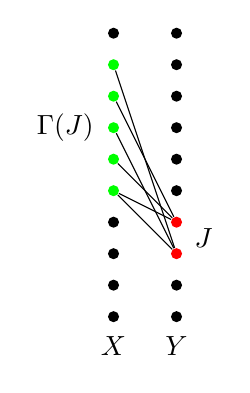
\begin{tikzpicture}[grow = right]
    \node [start]{}
    	child foreach \i in {10, 9}{
            node [end] (x\i) {}
               	child [end]{
	             	node [end] (y\i){}
    	            edge from parent [opacity = 0]
        	    }
            edge from parent [opacity = 0]
        }
        child foreach \i in {8, ..., 7}{
            node [end] (x\i) {}
               	child [endY]{
	             	node [endY] (y\i){}
    	            edge from parent [opacity = 0]
        	    }
            edge from parent [opacity = 0]
        }
        child foreach \i in {6, ..., 2}{
            node [endG] (x\i) {}
               	child [end]{
	             	node [end] (y\i){}
    	            edge from parent [opacity = 0]
        	    }
            edge from parent [opacity = 0]
        }
        child {
        	node [end] (x1) {}
           		child [end]{
	          		node [end] (y1){}
	    	        edge from parent [opacity = 0]
                }
    	   	edge from parent [opacity = 0]
        };

	\path [edge](y8) -- (x6);
    \path [edge](y8) -- (x4);
    \path [edge](y8) -- (x2);
    \path [edge](y7) -- (x3);
    \path [edge](y7) -- (x5);
    \path [edge](y7) -- (x6);

    \node at (x10.south) [below = 0.05cm] {$X$};
    \node at (y10.south) [below = 0.05cm] {$Y$};

    \path [opacity = 0](y7) -- (y8) node [start, midway] (mid){};
    \node <.(2)-> at (mid.east) [right = 0.05cm] {$J$};
    \node <.(3)-> at (x4.west) [left = 0.05cm] {$\Gamma(J)$};
\end{tikzpicture}
        \end{column}

        \pause
        \pause
        \pause
        \begin{column}{5cm}
            \begin{itemize}
                \item $\forall y \in Y ~~ deg(y) = d$
            	\pause
	            \item $\forall J \subset Y, ~
            		|J| < r \Rightarrow \Gamma(J) \ge \frac{2}{3}d|J|$
            \end{itemize}
		\end{column}
    \end{columns}

    \pause
    In fact we are unable to check this properties in polynomial time.

\end{frame}

\begin{frame}
	\frametitle{Our results}

	$P(x_1, \ldots, x_d) = x_1 \oplus x_2 \oplus \ldots \oplus x_{d - k} \oplus 
	Q(x_{d - k + 1}, \ldots, x_d)$, $Q$ --- arbitrary.

	\pause
	\begin{theorem}
		There are exist an explicit construction of graph $G$ such, that:
		\begin{itemize}
			\item $\forall$ myopic algorithms $A$,
        		 $\Pr\limits_{x, r}[t(A(G, P, b)) \ge 2^{\Omega(n)}] \ge 1 - 2^{-\Omega(n)}$
		\end{itemize}
	\end{theorem}

    \pause
    \begin{itemize}
	    \item Explicit (or random) graph $G$.
    	\pause
    	\item $K = n^{1 - \epsilon}$
    	\pause
    	\item Much simpler than in previous work.
    \end{itemize}
\end{frame}

\begin{frame}
    \frametitle{Graph constrution}

    \pause
    \tikzstyle{end} = [circle, minimum width = 4pt, fill, inner sep = 1pt,
	opacity = 1]
\tikzstyle{start} = [circle, inner sep = 1pt, opacity = 0]

\onslide<1->{
\tikzstyle{end3} = [circle, minimum width = 4pt, fill, inner sep = 1pt,
	opacity = 0]
%\tikzstyle{end5} = [circle, minimum width = 4pt, fill, inner sep = 1pt,
%	opacity = 0]
}

\only<3->{
	\tikzstyle{end3} = [circle, minimum width = 4pt, fill, inner sep = 1pt,
		opacity = 1]
}
%\only<5->{
	\tikzstyle{end5} = [color = red, circle, minimum width = 4pt, fill, inner sep = 1pt,
		opacity = 1]
%}
            
\tikzstyle{level 1} = [level distance = 0.1cm, sibling distance = 0.4cm]
\tikzstyle{level 2} = [level distance = 0.8cm]
\tikzstyle{level 3} = [level distance = 1cm]
\tikzstyle{level 4} = [level distance = 0.4cm]

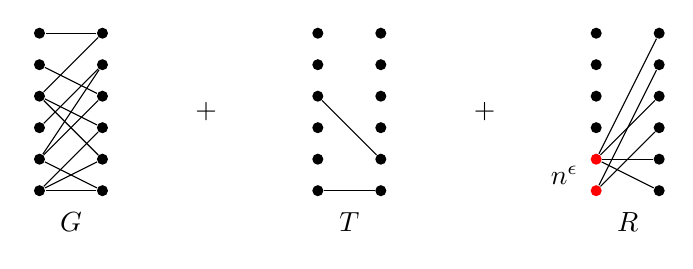
\begin{tikzpicture}[grow = right]
    \node [start]{}
    	child foreach \i in {6, ..., 1}{
            node [end] (x\i) {}
               	child [end]{
	             	node [end] (y\i){}
    	            edge from parent [opacity = 0]
        	    }
            edge from parent [opacity = 0]
        };

    \path [draw, opacity = 1](y1) -- (x3);
    \path [draw, opacity = 1](y1) -- (x1);
    \path [draw, opacity = 1](y2) -- (x4);
    \path [draw, opacity = 1](y2) -- (x5);
    \path [draw, opacity = 1](y3) -- (x5);
    \path [draw, opacity = 1](y3) -- (x2);
    \path [draw, opacity = 1](y4) -- (x3);
    \path [draw, opacity = 1](y4) -- (x6);
    \path [draw, opacity = 1](y5) -- (x3);
    \path [draw, opacity = 1](y5) -- (x6);
    \path [draw, opacity = 1](y6) -- (x5);
    \path [draw, opacity = 1](y6) -- (x6);

    \path [opacity = 0](y6) -- (x6) node [start, midway] (mid){};
    \node at (mid.south) [below = 0.1cm] {$G$};

    \path [opacity = 0](y3) -- (y4) node [start, midway] (mid2){};
    \node <.(2)-> at (mid2.east) [right = 1cm] (plus) {$+$};

    \node <.(3)-> at (plus.east) [right = 1cm, start]{}
    	child foreach \i in {6, ..., 1}{
            node [end3] (xx\i) {}
               	child [end3]{
	             	node [end3] (yy\i){}
    	            edge from parent [opacity = 0]
        	    }
            edge from parent [opacity = 0]
        };

    \path <.(3)-> [draw, opacity = 1](yy5) -- (xx3);
    \path <.(3)-> [draw, opacity = 1](yy6) -- (xx6);

    \path <.(3)-> [opacity = 0](yy6) -- (xx6) node [start, midway] (mid){};
    \node <.(3)-> at (mid.south) [below = 0.1cm] {$T$};

    \path <.(3)-> [opacity = 0](yy3) -- (yy4) node [start, midway] (mid3){};
    \node <.(4)-> at (mid3.east) [right = 1cm] (plus2) {$+$};

    \node <.(5)-> at (plus2.east) [right = 1cm, start]{}
    	child foreach \i in {6, 5}{
            node [end5] (xxx\i) {}
               	child [end]{
	             	node [end] (yyy\i){}
    	            edge from parent [opacity = 0]
        	    }
            edge from parent [opacity = 0]
        }
        child foreach \i in {4, ..., 1}{
            node [end] (xxx\i) {}
               	child [end]{
	             	node [end] (yyy\i){}
    	            edge from parent [opacity = 0]
        	    }
            edge from parent [opacity = 0]
        };

    \path <.(5)-> [draw, opacity = 1](xxx5) -- (yyy1);
    \path <.(5)-> [draw, opacity = 1](xxx6) -- (yyy2);
    \path <.(5)-> [draw, opacity = 1](xxx5) -- (yyy3);
    \path <.(5)-> [draw, opacity = 1](xxx6) -- (yyy4);
    \path <.(5)-> [draw, opacity = 1](xxx5) -- (yyy5);
    \path <.(5)-> [draw, opacity = 1](xxx5) -- (yyy6);

    \path <.(5)-> [opacity = 0](yyy6) -- (xxx6) node [start, midway] (mid3){};
    \node <.(5)-> at (mid3.south) [below = 0.1cm] {$R$};

    \path <.(5)-> [opacity = 0](xxx6) -- (xxx5) node [start, midway] (mid4){};
    \node <.(5)-> at (mid4.west) [left = 0.05cm] {$n^{\epsilon}$};
\end{tikzpicture}


    \begin{itemize}
	    \item $G$ is an expander;
   		\pause
        \pause
        \item $G + T$ has full rank. $\forall y \in Y \subset T, ~
		    deg(y) = 1$;
        \pause
        \pause
        \item $R$ contains unlinear edges. $|\{x \mid x \in X, ~ deg(x)
		    \ne 0\}| \le n^{\epsilon}$.
    \end{itemize}
\end{frame}

\begin{frame}
	\frametitle{Proof plan}

	\begin{itemize}
		\pause
		\item Lower bounds for unsatisfiable formulas.
		\pause
		\item With probability $2^{-\Omega(n)}$ after several step
    		partial subtitution matches with concrete satisfying
            assignment.
	\end{itemize}
   
\end{frame}